\pdfoutput=1
\documentclass[a4paper,pdftex,10pt]{article}
% \usepackage[whole,autotilde]{bxcjkjatype}
\usepackage[T1]{fontenc}
\usepackage{tgtermes}

% ---Display \subsubsection at the Index
\setcounter{tocdepth}{3}

% ---Setting about the geometry of the document----
\usepackage{a4wide}
% \pagestyle{empty}

% ---Physics and Math Packages---
\usepackage{amssymb,amsfonts,amsthm,mathtools}
\usepackage{physics,braket,bm,slashed}

% ---underline---
\usepackage[normalem]{ulem}

% ---cancel---
\usepackage{cancel}

% --- surround the texts or equations
\usepackage{fancybox,ascmac}

% ---settings of theorem environment---
\theoremstyle{definition}
\newtheorem{dfn}{Definition}
\newtheorem{prop}{Proposition}
\newtheorem{thm}{Theorem}

% ---settings of proof environment---
\renewcommand{\proofname}{\textbf{Proof}}
\renewcommand{\qedsymbol}{$\blacksquare$}

% ---Ignore the Warnings---
\usepackage{silence}
\WarningFilter{latexfont}{Some font shapes,Font shape}
\ExplSyntaxOn
\msg_redirect_name:nnn{hooks}{generic-deprecated}{none}
\ExplSyntaxOff

% ---Insert the figure (If insert the `draft' at the option, the process becomes faster.)---
% \usepackage{graphicx}
% \usepackage{subcaption}

% ----Add a link to a text---
\usepackage{url,hyperref}
\usepackage[dvipsnames,svgnames]{xcolor}
\hypersetup{colorlinks=true,citecolor=FireBrick,linkcolor=Navy,urlcolor=purple}

% ---Tikz---
\usepackage{tikz,pgf,pgfplots,circuitikz}
\pgfplotsset{compat=1.15}
\usetikzlibrary{intersections, arrows.meta, angles, calc, 3d, decorations.pathmorphing}
\usepackage[compat=1.1.0]{tikz-feynhand}

% ---tcolorbox---
\usepackage{tcolorbox}
\tcbuselibrary{raster,skins,breakable}
\newtcolorbox{graybox}[1][]{frame empty, colback=black!07!white, sharp corners}

% ---Add the section number to the equation, figure, and table number---
\makeatletter
   \renewcommand{\theequation}{$\thesection.\arabic{equation}$}
   \@addtoreset{equation}{section}
   
   \renewcommand{\thefigure}{\thesection.\arabic{figure}}
   \@addtoreset{figure}{section}
   
   \renewcommand{\thetable}{\thesection.\arabic{table}}
   \@addtoreset{table}{section}
\makeatother

% ---enumerate---
% \renewcommand{\labelenumi}{$\arabic{enumi}.$}
% \renewcommand{\labelenumii}{$(\arabic{enumii})$}

% ---Index---
% \usepackage{makeidx}
% \makeindex 

% ---footnotes---
\renewcommand{\thefootnote}{$\ast$\arabic{footnote}}

% ---Title---
\title{Notes on Anomalies}
\author{Itsuki Miyane}
\date{Last modified:\ \today}

\begin{document}

\maketitle

*In this report, I use Mathematica for heavy calculations. I will omit "massive" computations, such as the derivation of Christoffel symbols and covariant derivatives, etc.

\begin{enumerate}
  \item
        The background line element
        \begin{equation}
          \dd s^2
          =
          -
          \left( 1-\frac{2\mu}{r} \right)\dd t^2
          +
          \left( 1-\frac{2\mu}{r} \right)^{-1}\dd r^2
          +
          r^2
          (\dd\theta^2+\sin^2\theta\dd\varphi^2)
        \end{equation}
        implies the metric is obtained as
        \begin{equation}
          g_{\mu\nu}
          =
          \begin{pmatrix}
            -\left( 1-2\mu/r \right) & 0                            & 0   & 0               \\
            0                        & \left( 1-2\mu/r \right)^{-1} & 0   & 0               \\
            0                        & 0                            & r^2 & 0               \\
            0                        & 0                            & 0   & r^2\sin^2\theta
          \end{pmatrix}
          .
        \end{equation}
        Thus, we find the inverse
        \begin{equation}
          g^{\mu\nu}
          =
          \begin{pmatrix}
            -(1-2\mu/r)^{-1} & 0        & 0     & 0                  \\
            0                & 1-2\mu/r & 0     & 0                  \\
            0                & 0        & 1/r^2 & 0                  \\
            0                & 0        & 0     & 1/r^2 \sin^2\theta
          \end{pmatrix}
        \end{equation}
        and Christoffel symbols are given by
        \begin{equation}
          \begin{array}{lll}
            \Gamma^{t}_{\ tr}
            =
            \Gamma^{t}_{\ rt}
            =
            \frac{\mu/r}{1-2\mu/r}
            ,
             &
            \Gamma^{r}_{\ tt}
            =
            \frac{\mu(1-2\mu r)}{r^2}
            ,
             &
            \Gamma^{r}_{\ rr}
            =
            -\frac{\mu}{r^2(1-2\mu r)}
            ,
            \\
            \Gamma^{r}_{\ \theta\theta}
            =
            -r\left( 1-\frac{2\mu}{r} \right)
            ,
             &
            \Gamma^{r}_{\ \varphi\varphi}
            =
            -r\left( 1-\frac{2\mu}{r} \right)\sin^2\theta
            ,
             &
            \Gamma^{\theta}_{\ r\theta}
            =
            \Gamma^{\theta}_{\ \theta r}
            =
            \frac{1}{r}
            ,
            \\
            \Gamma^{\theta}_{\ \varphi\varphi}
            =
            -\cos\theta\sin\theta
            ,
             &
            \Gamma^{\varphi}_{\ r\varphi}
            =
            \Gamma^{\varphi}_{\ \varphi r}
            =
            \frac{1}{r}
            ,
             &
            \Gamma^{\varphi}_{\ \varphi\theta}
            =
            \Gamma^{\varphi}_{\ \theta\varphi}
            =
            \frac{1}{\tan\theta}
          \end{array}
        \end{equation}
        and otherwise are zero. By using these results, we get the Klein-Gordon equation as
        \begin{align}
          g^{\mu\nu}\nabla_{\mu}\nabla_{\nu}
          \Phi
           & =
          g^{\mu\nu}
          (\partial_{\mu}\partial_{\nu}\Phi-\Gamma^{\rho}_{\ \mu\nu}\partial_{\rho}\Phi)
          \nonumber
          \\
           &
          =
          \frac{2}{r}\left( 1-\frac{\mu}{r} \right)\pdv{\Phi}{r}
          +
          \left( 1-\frac{2\mu}{r} \right)\pdv[2]{\Phi}{r}
          -
          \frac{1}{1-2\mu/r}\pdv[2]{\Phi}{t}
          \nonumber
          \\
           & \qquad
          +
          \frac{1}{r^2}
          \left[
            \frac{1}{\tan\theta}\pdv{\Phi}{\theta}
            +
            \pdv[2]{\Phi}{\theta}
            +
            \frac{1}{\sin^2\theta}\pdv[2]{\Phi}{\theta}
            \right]
          .
          \label{eqn:1.1}
        \end{align}
        We will insert the expression
        \begin{equation}
          \Phi(x)
          =
          \frac{1}{r}\phi(t,r)Y_{lm}(\theta,\varphi)
          \label{eqn:1.2_expansion}
        \end{equation}
        where $Y_{lm}(\theta.\varphi)$ is a spherical harmonics which satisfies the following relation:
        \begin{equation}
          \frac{1}{r^2}
          \left[
            \frac{1}{\tan\theta}\pdv{}{\theta}
            +
            \pdv[2]{}{\theta}
            +
            \frac{1}{\sin^2\theta}\pdv[2]{}{\theta}
            \right]
          Y_{lm}(\theta,\varphi)
          =
          -
          \frac{l(l+1)}{r^2}
          Y_{lm}(\theta,\varphi)
          .
        \end{equation}
        Putting the expansion \eqref{eqn:1.2_expansion} into \eqref{eqn:1.1}, each term becomes
        \begin{align}
          \frac{2}{r}\left( 1-\frac{\mu}{r} \right)\pdv{\Phi}{r}
           & =
          \frac{2}{r}\left( 1-\frac{\mu}{r} \right)
          \left[ -\frac{\phi}{r^2}+\frac{1}{r}\pdv{\phi}{r} \right]Y_{lm}
          \label{eqn:1.3}
          \\
          \left( 1-\frac{2\mu}{r} \right)\pdv[2]{\Phi}{r}
           & =
          \left( 1-\frac{2\mu}{r} \right)
          \left( \frac{2\phi}{r^3}-\frac{2}{r^2}\pdv{\phi}{r}+\frac{1}{r}\pdv[2]{\phi}{r} \right)Y_{lm}
          \label{eqn:1.4}
          \\
          \frac{1}{1-2\mu/r}\pdv[2]{\Phi}{t}
           & =
          \frac{1}{r(1-2\mu/r)}\pdv[2]{\phi}{t}Y_{lm}
          .
        \end{align}
        Merging two equalities \eqref{eqn:1.3}, \eqref{eqn:1.4}, the sum becomes
        \begin{align}
           & \hspace*{10pt}
          \frac{2}{r}\left( 1-\frac{\mu}{r} \right)
          \left[ -\frac{\phi}{r^2}+\frac{1}{r}\pdv{\phi}{r} \right]
          +
          \left( 1-\frac{2\mu}{r} \right)
          \left( \frac{2\phi}{r^3}-\frac{2}{r^2}\pdv{\phi}{r}+\frac{1}{r}\pdv[2]{\phi}{r} \right)
          \nonumber
          \\
           & =
          -\frac{2\mu}{r^4}\phi
          +
          \frac{2\mu}{r^3}\pdv{\phi}{r}
          +
          \frac{1}{r}\pdv[2]{\phi}{r}
          -
          \frac{2\mu}{r^2}\pdv[2]{\phi}{r}
          \nonumber
          \\
           & =
          -
          \frac{2\mu}{r^4}\phi
          +
          \frac{1}{r}\pdv{}{r}\left[ \left( 1-\frac{2\mu}{r} \right)\pdv{\phi}{r} \right]
        \end{align}
        where we omit the overall factor $Y_{lm}$. Thus we obtain equality as
        \begin{equation}
          -
          \frac{2\mu}{r^4}\phi
          +
          \frac{1}{r}\pdv{}{r}\left[ \left( 1-\frac{2\mu}{r} \right)\pdv{\phi}{r} \right]
          -
          \frac{1}{r(1-2\mu/r)}\pdv[2]{\phi}{t}
          -
          \frac{l(l+1)}{r^3}\phi
          =
          0
        \end{equation}
        and finally
        \begin{equation}
          \pdv[2]{\phi}{t}
          -
          \left( 1-\frac{2\mu}{r} \right)\pdv{}{r}\left[ \left( 1-\frac{2\mu}{r} \right)\pdv{\phi}{r} \right]
          +
          \left( 1-\frac{2\mu}{r} \right)
          \left[ \frac{2\mu}{r^3}+\frac{l(l+1)}{r^2} \right]\phi
          =
          0
          .
        \end{equation}
        Thus, the effective potential is given by
        \begin{equation}
          V(r)
          =
          \left( 1-\frac{2\mu}{r} \right)
          \left[ \frac{2\mu}{r^3}+\frac{l(l+1)}{r^2} \right]
          .
        \end{equation}

  \item
  If we assume $l\gg 1$, we can rewrite the potential
  \begin{equation}
    V(r)
    \sim
    l(l+1)\left( \frac{1}{r^2}-\frac{2\mu}{r^3} \right)
  \end{equation}
  effectively and this potential has the minimum at 
  \begin{equation}
    r_{m}
    =
    3\mu
    .
  \end{equation}

  \begin{figure}[ht]
    \centering
    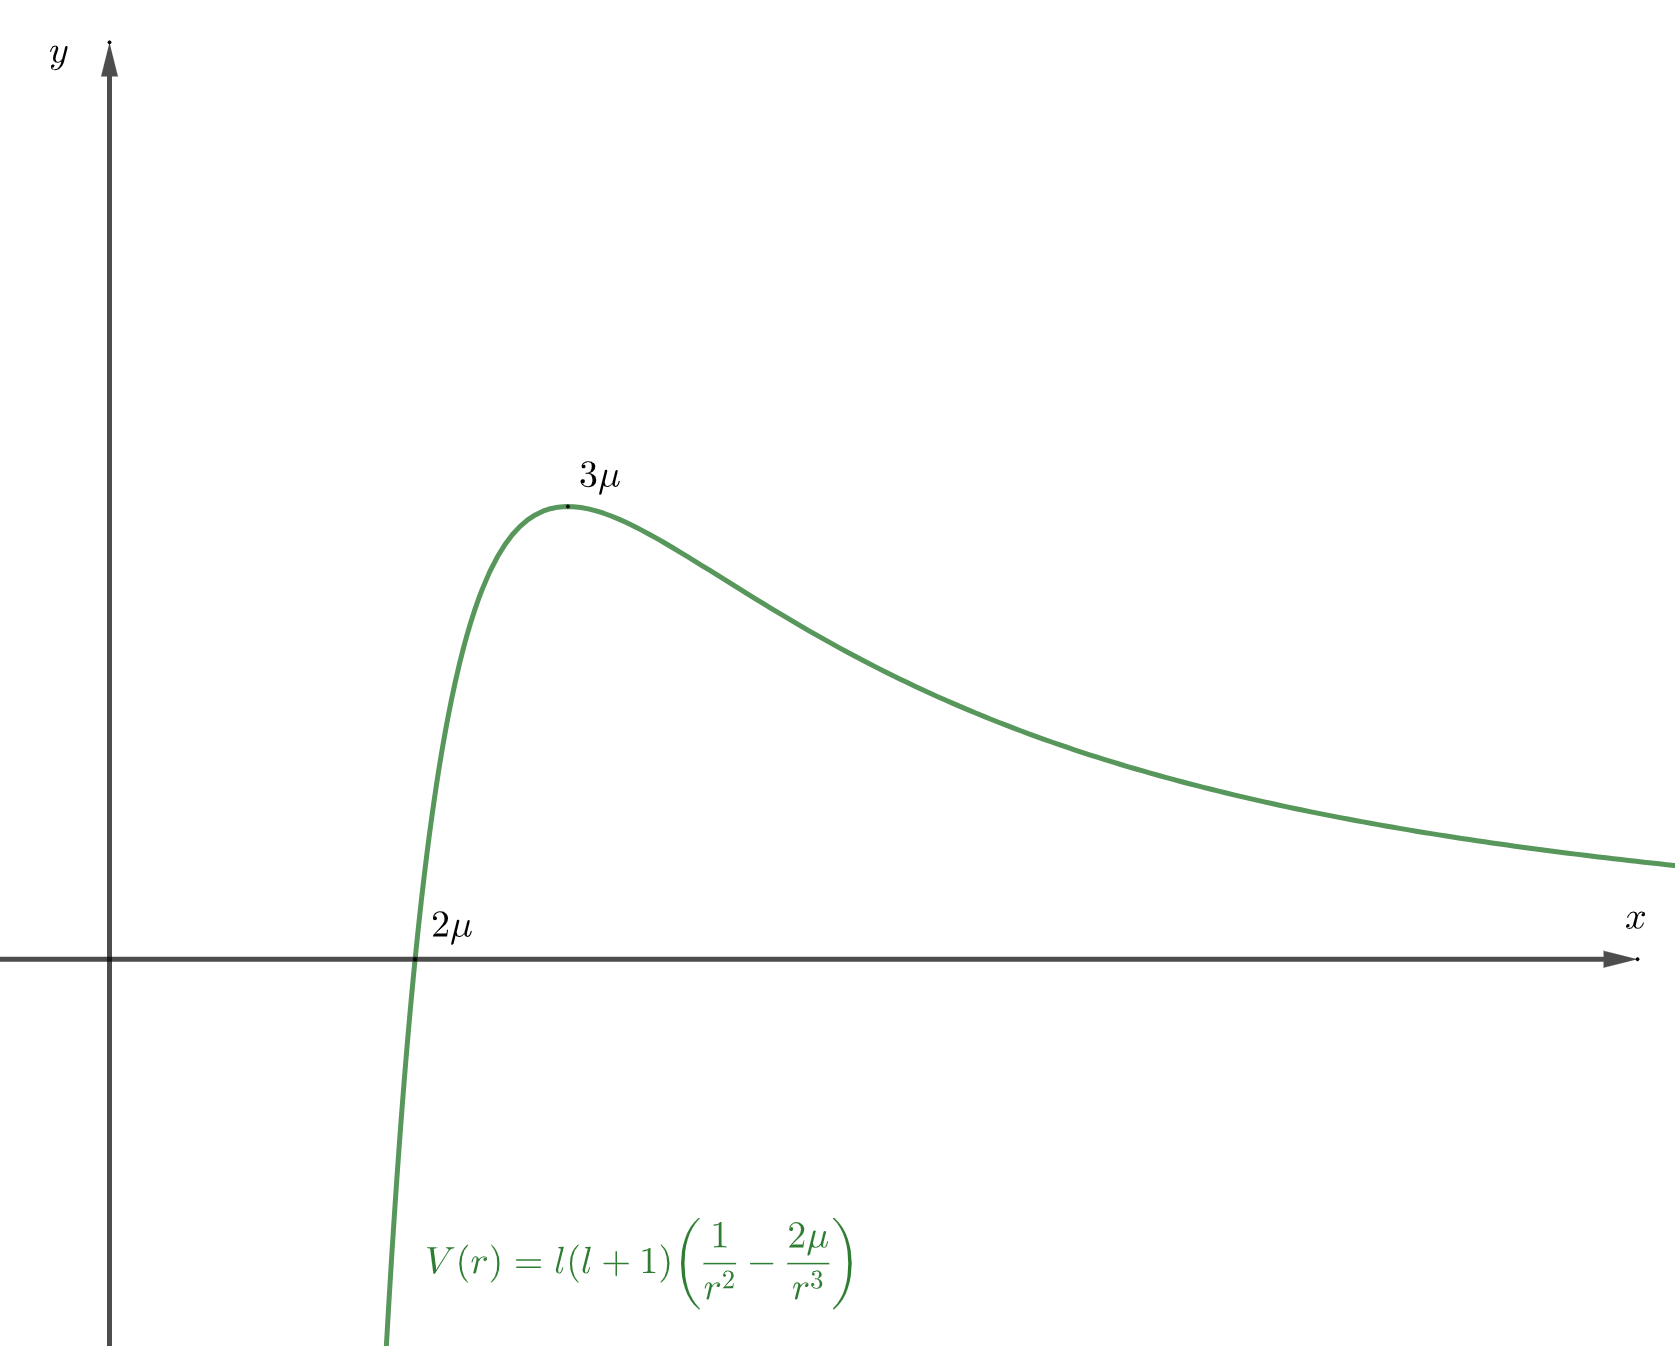
\includegraphics[width=0.8\textwidth]{potential.PNG}
    \caption{Potential $V(r)$ in the limit $l\gg 1$}
  \end{figure}

  Let us consider the radius of a photon sphere $r_{p}$. It has already been given in Lecture 7 as 
  \begin{equation}
    r_{p}
    =
    3\mu
    .
  \end{equation}
  Therefore, the result is, of course, $r_{m}=r_{p}$.

\end{enumerate}

\begin{thebibliography}{99}
  \bibitem{Wald:1984}
  R. M. Wald, \textit{General Relativity}, University of Chicago Press, Chicago (1984).
  \bibitem{stack01}
  "\href{https://physics.stackexchange.com/questions/313336/klein-gordon-equation-in-schwarzschild-spacetime-spherical-harmonic-mode-expans}{\textit{Klein Gordon equation in Schwarzschild spacetime (spherical harmonic mode expansion)}}", StackExchange. (Last access: May 12, 2024)
\end{thebibliography}

% ----------------------------------------
% \appendix
% \section{The computation of the radius of the photon sphere}











% ----------------------------------------
% \clearpage
% \bibliography{ref}
% \bibliographystyle{ytamsalpha}

% ----------------------------------------
% \clearpage
% \index{hoge@hoge}
% \printindex

\end{document}
